\documentclass[twoside,11pt]{article}

% Any additional packages needed should be included after jmlr2e. Note that
% jmlr2e.sty includes epsfig, amssymb, natbib and graphicx, and defines many
% common macros, such as 'proof' and 'example'.
%
% It also sets the bibliographystyle to plainnat; for more information on natbib
% citation styles, see the natbib documentation, a copy of which is archived at
% http://www.jmlr.org/format/natbib.pdf

\usepackage{artifacts/jmlr2e}

\usepackage[utf8]{inputenc}
\usepackage[english]{babel}
\usepackage[T1]{fontenc}

\usepackage{xcolor}
\definecolor{halfgray}{gray}{0.55}
\definecolor{ipython_frame}{RGB}{207, 207, 207}
\definecolor{ipython_bg}{RGB}{247, 247, 247}
\definecolor{ipython_red}{RGB}{186, 33, 33}
\definecolor{ipython_green}{RGB}{0, 128, 0}
\definecolor{ipython_cyan}{RGB}{64, 128, 128}
\definecolor{ipython_purple}{RGB}{170, 34, 255}

\usepackage{listings}
\lstset{
    breaklines=true,
    %
    extendedchars=true,
    literate=
    {á}{{\'a}}1 {é}{{\'e}}1 {í}{{\'i}}1 {ó}{{\'o}}1 {ú}{{\'u}}1
    {Á}{{\'A}}1 {É}{{\'E}}1 {Í}{{\'I}}1 {Ó}{{\'O}}1 {Ú}{{\'U}}1
    {à}{{\`a}}1 {è}{{\`e}}1 {ì}{{\`i}}1 {ò}{{\`o}}1 {ù}{{\`u}}1
    {À}{{\`A}}1 {È}{{\'E}}1 {Ì}{{\`I}}1 {Ò}{{\`O}}1 {Ù}{{\`U}}1
    {ä}{{\"a}}1 {ë}{{\"e}}1 {ï}{{\"i}}1 {ö}{{\"o}}1 {ü}{{\"u}}1
    {Ä}{{\"A}}1 {Ë}{{\"E}}1 {Ï}{{\"I}}1 {Ö}{{\"O}}1 {Ü}{{\"U}}1
    {â}{{\^a}}1 {ê}{{\^e}}1 {î}{{\^i}}1 {ô}{{\^o}}1 {û}{{\^u}}1
    {Â}{{\^A}}1 {Ê}{{\^E}}1 {Î}{{\^I}}1 {Ô}{{\^O}}1 {Û}{{\^U}}1
    {œ}{{\oe}}1 {Œ}{{\OE}}1 {æ}{{\ae}}1 {Æ}{{\AE}}1 {ß}{{\ss}}1
    {ç}{{\c c}}1 {Ç}{{\c C}}1 {ø}{{\o}}1 {å}{{\r a}}1 {Å}{{\r A}}1
    {€}{{\EUR}}1 {£}{{\pounds}}1
}

%%
%% Python definition (c) 1998 Michael Weber
%% Additional definitions (2013) Alexis Dimitriadis
%% modified by me (should not have empty lines)
%%
\lstdefinelanguage{iPython}{
    morekeywords={access,and,break,class,continue,def,del,elif,else,except,exec,finally,for,from,global,if,import,in,is,lambda,not,or,pass,print,raise,return,try,while},%
    %
    % Built-ins
    morekeywords=[2]{abs,all,any,basestring,bin,bool,bytearray,callable,chr,classmethod,cmp,compile,complex,delattr,dict,dir,divmod,enumerate,eval,execfile,file,filter,float,format,frozenset,getattr,globals,hasattr,hash,help,hex,id,input,int,isinstance,issubclass,iter,len,list,locals,long,map,max,memoryview,min,next,object,oct,open,ord,pow,property,range,raw_input,reduce,reload,repr,reversed,round,set,setattr,slice,sorted,staticmethod,str,sum,super,tuple,type,unichr,unicode,vars,xrange,zip,apply,buffer,coerce,intern},%
    %
    sensitive=true,%
    morecomment=[l]\#,%
    morestring=[b]',%
    morestring=[b]",%
    %
    morestring=[s]{'''}{'''},% used for documentation text (mulitiline strings)
    morestring=[s]{"""}{"""},% added by Philipp Matthias Hahn
    %
    morestring=[s]{r'}{'},% `raw' strings
    morestring=[s]{r"}{"},%
    morestring=[s]{r'''}{'''},%
    morestring=[s]{r"""}{"""},%
    morestring=[s]{u'}{'},% unicode strings
    morestring=[s]{u"}{"},%
    morestring=[s]{u'''}{'''},%
    morestring=[s]{u"""}{"""},%
    %
    % {replace}{replacement}{lenght of replace}
    % *{-}{-}{1} will not replace in comments and so on
    literate=
    *{+}{{{\color{ipython_purple}+}}}1
    {-}{{{\color{ipython_purple}-}}}1
    {*}{{{\color{ipython_purple}$^\ast$}}}1
    {/}{{{\color{ipython_purple}/}}}1
    {^}{{{\color{ipython_purple}\^{}}}}1
    {?}{{{\color{ipython_purple}?}}}1
    {!}{{{\color{ipython_purple}!}}}1
    {\%}{{{\color{ipython_purple}\%}}}1
    {<}{{{\color{ipython_purple}<}}}1
    {>}{{{\color{ipython_purple}>}}}1
    {|}{{{\color{ipython_purple}|}}}1
    {\&}{{{\color{ipython_purple}\&}}}1
    {~}{{{\color{ipython_purple}~}}}1
    %
    {==}{{{\color{ipython_purple}==}}}2
    {<=}{{{\color{ipython_purple}<=}}}2
    {>=}{{{\color{ipython_purple}>=}}}2
    %
    {+=}{{{+=}}}2
    {-=}{{{-=}}}2
    {*=}{{{$^\ast$=}}}2
    {/=}{{{/=}}}2,
    %
    literate=
    {á}{{\'a}}1 {é}{{\'e}}1 {í}{{\'i}}1 {ó}{{\'o}}1 {ú}{{\'u}}1
    {Á}{{\'A}}1 {É}{{\'E}}1 {Í}{{\'I}}1 {Ó}{{\'O}}1 {Ú}{{\'U}}1
    {à}{{\`a}}1 {è}{{\`e}}1 {ì}{{\`i}}1 {ò}{{\`o}}1 {ù}{{\`u}}1
    {À}{{\`A}}1 {È}{{\'E}}1 {Ì}{{\`I}}1 {Ò}{{\`O}}1 {Ù}{{\`U}}1
    {ä}{{\"a}}1 {ë}{{\"e}}1 {ï}{{\"i}}1 {ö}{{\"o}}1 {ü}{{\"u}}1
    {Ä}{{\"A}}1 {Ë}{{\"E}}1 {Ï}{{\"I}}1 {Ö}{{\"O}}1 {Ü}{{\"U}}1
    {â}{{\^a}}1 {ê}{{\^e}}1 {î}{{\^i}}1 {ô}{{\^o}}1 {û}{{\^u}}1
    {Â}{{\^A}}1 {Ê}{{\^E}}1 {Î}{{\^I}}1 {Ô}{{\^O}}1 {Û}{{\^U}}1
    {œ}{{\oe}}1 {Œ}{{\OE}}1 {æ}{{\ae}}1 {Æ}{{\AE}}1 {ß}{{\ss}}1
    {ç}{{\c c}}1 {Ç}{{\c C}}1 {ø}{{\o}}1 {å}{{\r a}}1 {Å}{{\r A}}1
    {€}{{\EUR}}1 {£}{{\pounds}}1,
    %
%   identifierstyle=\color{red}\ttfamily,
    commentstyle=\color{ipython_cyan}\ttfamily,
    stringstyle=\color{ipython_red}\ttfamily,
    keepspaces=true,
    showspaces=false,
    showstringspaces=false,
    %
    rulecolor=\color{ipython_frame},
    frame=single,
    frameround={t}{t}{t}{t},
    framexleftmargin=6mm,
    numbers=left,
    numberstyle=\tiny\color{halfgray},
    %
    %
    backgroundcolor=\color{ipython_bg},
    %   extendedchars=true,
    basicstyle=\scriptsize\ttfamily,
    keywordstyle=\color{ipython_green}\ttfamily,
}

% Definitions of handy macros can go here

\newcommand{\dataset}{{\cal D}} \newcommand{\fracpartial}[2]{\frac{\partial
#1}{\partial  #2}}

% Heading arguments are {volume}{year}{pages}{date submitted}{date
% published}{paper id}{author-full-names}

\jmlrheading{}{2022}{}{}{}{}{Georgios Douzas, and Fernando Bacao}

% Short headings should be running head and authors last names

\ShortHeadings{geometric-smote - A Package for Flexible and Efficient
Over-Sampling}{Douzas and Bacao}
\firstpageno{1}

\begin{document}

\title{geometric-smote - A Package for Flexible and Efficient Over-Sampling}

\author{\name Georgios Douzas \email gdouzas@novaims.unl.pt \\
       \addr NOVA Information Management School\\
       Universidade Nova de Lisboa\\
       Campus de Campolide, 1070-312 Lisboa, Portugal \AND \name Fernando Bacao
       \email bacao@novaims.unl.pt \\
       \addr NOVA Information Management School\\
       Universidade Nova de Lisboa\\
       Campus de Campolide, 1070-312 Lisboa, Portugal}

\editor{}

\maketitle

\begin{abstract}%   <- trailing '%' for backward compatibility of .sty file
	Learning from class-imbalanced data continues to be a frequent and
	challenging problem in machine learning. To mitigate this problem several
	approaches have been proposed. A popular approach is the generation of
	artificial data for the minority classes, known as over-sampling. Geometric
	SMOTE is a state-of-the-art over-sampling algorithm that has been shown to
	outperform other standard over-samplers in a large number of data sets. In
	order to make available Geometric SMOTE to the machine learning community,
	we provide a Python implementation with source code and documentation found
	at \url{https://github.com/georgedouzas/geometric-smote} and
	\url{https://geometric-smote.readthedocs.io}, respectively. The
	implementation integrates seamlessly with the \texttt{scikit-learn}
	ecosystem.
\end{abstract}

\begin{keywords}
  machine learning, classification, imbalanced learning, over-sampling, Python
\end{keywords}

\section{Introduction}

The imbalanced learning problem is defined as a machine learning classification
task using data sets with binary or multi-class targets where one of the
classes, called the majority class, outnumbers significantly the remaining
classes, called the minority class(es)~\citep{Chawla2003}. The imbalance
learning problem can be found in multiple domains such as chemical and
biochemical engineering, financial management, information technology, security,
business, agriculture or emergency management~\citep{Haixiang2017}. 

Standard machine learning classification algorithms induce a bias towards the
majority class during training. This results in low performance when metrics
suitable for imbalanced data are used for the classifier's evaluation.

In this paper, we present the \texttt{geometric-smote} software project, a
Python implementation of the Geometric-SMOTE~\citep{Douzas2019} algorithm. The
following sections provide a description of the algorithm's properties as well
as a presentation of the software architecture and functionalities.

\section{Geometric SMOTE algorithm}
\label{oversampling}

A general approach to deal with the imbalanced learning problem is the
modification at the data level by over-sampling the minority
class(es)~\citep{Fernandez2013}. Synthetic Minority Oversampling Technique
(SMOTE)~\citep{Chawla2002}, the first informed over-sampling algorithm proposed,
generates synthetic instances along a line segment that joins minority class
samples. Many variants of SMOTE have been proposed to deal with some of its
limitations~\citep{He2009}. A Python implementation of SMOTE and several of its
variants is available in the \texttt{imbalanced-learn}~\citep{Lemaitre2016}
toolbox, which is fully compatible with the popular machine learning library
\texttt{scikit-learn}~\citep{Pedregosa2011}.

Geometric SMOTE (G-SMOTE) uses a different approach compared to the existing
SMOTE's variations. More specifically, G-SMOTE over-sampling algorithm
substitutes the data generation mechanism of SMOTE by defining a flexible
geometric region around each minority class instance and generating synthetic
instances inside the boundaries of this region. The algorithm requires the
selection of the hyperparameters \texttt{truncation\_factor},
\texttt{deformation\_factor}, \texttt{selection\_strategy} and
\texttt{k\_neighbors}. The first three of them, called geometric
hyperparameters, control the shape of the geometric region while the later
adjusts its size. Figure \ref{fig:smote_vs_gsmote} presents a visual comparison
between the data generation mechanisms of SMOTE and G-SMOTE.

\begin{figure}
	\centering
	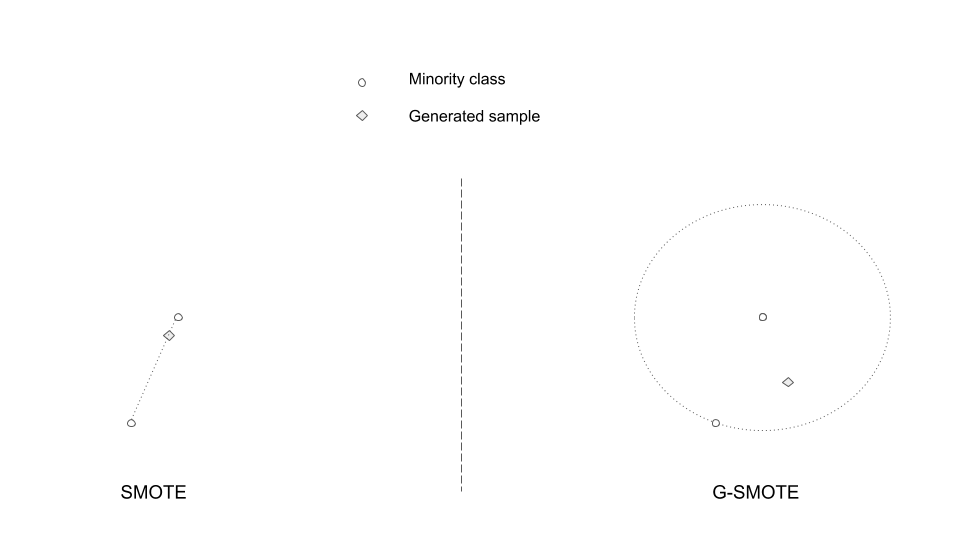
\includegraphics[width=1\linewidth]{artifacts/smote_vs_gsmote}
	\caption{Comparison between the data generation mechanisms of SMOTE and 
  G-SMOTE. SMOTE uses linear interpolation, while G-SMOTE defines a circle as the 
  permissible data generation area.}
	\label{fig:smote_vs_gsmote}
\end{figure}

G-SMOTE algorithm has been shown to outperform SMOTE and its variants across 69
imbalanced data sets for various classifiers and evaluation metrics
~\citep{Douzas2019}.

\section{Software architecture}

The \texttt{geometric-smote} software project is written in Python 3. It
contains an object-oriented implementation of G-SMOTE as well as an extensive
online documentation found at \url{https://geometric-smote.readthedocs.io}. The
provided API is compatible with \texttt{scikit-learn} and
\texttt{imbalanced-learn} libraries, therefore it makes full use of various
features that support standard machine learning functionalities. For instance,
\texttt{GeometricSMOTE} objects can be used in a machine learning pipelines,
through \texttt{imbalanced-learn}'s class \texttt{Pipeline}, that automatically
combines \texttt{samplers}, \texttt{transformers} and \texttt{estimators}.

The main module of \texttt{geometric-smote} is called
\texttt{geometric-smote.py}. It contains the class \texttt{GeometricSMOTE} that
implements the G-SMOTE algorithm. The initialization of a
\texttt{GeometricSMOTE} instance includes G-SMOTE's geometric hyperparameters
that control the generation of synthetic data i.e. \texttt{truncation\_factor},
\texttt{deformation\_factor} and \texttt{selection\_strategy}. The
implementation also supports the use of categorical features through the
\texttt{categorical\_features} initialization parameter.

\texttt{GeometricSMOTE} inherits from the \texttt{BaseOverSampler} class of
\texttt{imbalanced-learn} library and implements its \texttt{\_fit\_resample}
abstract method. Consequently, an instance of the \texttt{GeometricSMOTE} class
provides the \texttt{fit} and \texttt{fit\_resample} methods, the two main
methods for resampling. Both of them take as input parameters the \texttt{X} and
\texttt{y}. The first method computes various statistics which are used to
resample \texttt{X}, while the second method does the same but additionally
returns a resampled version of \texttt{X} and \texttt{y}. Figure
\ref{fig:class_diagram} provides a visual representation of the above classes
and functions hierarchy while Listing \ref{lst:snippet} presents an example of
over-sampling am imbalanced 3-class data set.

\begin{figure}
	\centering
	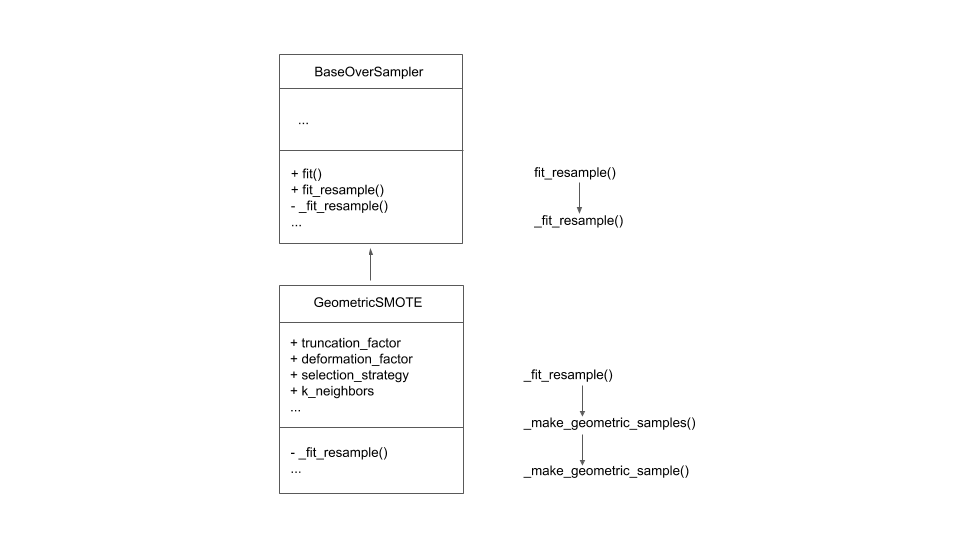
\includegraphics[width=1\linewidth]{artifacts/class_diagram}
	\caption{UML class diagrams and callgraphs of main classes and methods.}
	\label{fig:class_diagram}
\end{figure} 

\begin{lstlisting}[language={iPython}, caption={ Code snippet to over-sample a data set using G-SMOTE.}, captionpos=b, label={lst:snippet}]
from collections import Counter from gsmote
import GeometricSMOTE from sklearn.datasets import make_classification

# Generate an imbalanced 3-class data set
X, y = make_classification(
	random_state=23, 
	n_classes=3, 
	n_informative=5, 
	n_samples=500, 
	weights=[0.8,0.15, 0.05]
)

# Create a GeometricSMOTE object with default hyperparameters
gsmote = GeometricSMOTE()

# Resample the imbalanced data set using G-SMOTE
X_res, y_res = gsmote.fit_resample(X, y) 
\end{lstlisting}

\section{Project management}
Releases of the \texttt{geometric-smote} package are available via PyPI and
conda-forge. Collaboration on the project is possible via GitHub where users can
open new issues or reply to current issues and make pull requests. Continuous
integration with GitHub Actions is also supported. The \texttt{PEP8} style
standards are followed while extensive unit testing of the code is applied. The
documentation includes installation instructions, a detailed description of the
API and a user guide with various examples. Finally, the package is distributed
under the MIT license.

\section{Impact and conclusions}
The \texttt{geometric-smote} project provides the only Python implementation, to
the best of our knowledge, of the state-of-the-art over-sampling algorithm
G-SMOTE. A significant advantage of this implementation is that it is built on
top of the \texttt{scikit-learn}'s ecosystem. Therefore, using the G-SMOTE
over-sampler in typical machine learning workflows is an effortless task for the
user. Also, the public API of the main class \texttt{GeometricSMOTE} is
identical to the one implemented in \texttt{imbalanced-learn} for all
over-samplers. This means that users of \texttt{imbalanced-learn} and
\texttt{scikit-learn}, that apply over-sampling on imbalanced data, can
integrate the \texttt{gsmote} package in their existing work in a
straightforward manner or even replace directly any \texttt{imbalanced-learn}'s
over-sampler with \texttt{GeometricSMOTE}.

\vskip 0.2in
\bibliography{artifacts/references}

\end{document}
